\documentclass[letterpaper,twocolumn,10pt]{article}
\usepackage{usenix-2020-09}
\usepackage{graphicx}
\usepackage{booktabs}
\usepackage{url}
\usepackage{array}
\usepackage{tabularx}
\usepackage{tikz}
\usetikzlibrary{arrows.meta,positioning,calc}
\setlength{\parindent}{0pt}
\setlength{\parskip}{2pt}
\setlength{\emergencystretch}{3em}

\title{AI-Assisted Cryptographic Vulnerability Discovery in an Android APK}

\author{
{\rm Your Name(s)}\\
The University of Sydney
}

\date{}

\begin{document}
\maketitle

\begin{abstract}
We analyzed the provided Android APK to model authentication flows and assess security-sensitive randomness. We identified that session tokens are generated with \texttt{java.util.Random} and persisted as trusted session state in \texttt{SharedPreferences}. This is unsuitable for authentication. We provide code evidence, a realistic local attacker model, a concrete exploit path, and a mitigation based on \texttt{SecureRandom} and explicit session validation.
\end{abstract}

\section{Introduction}
APK analysis is required because Android apps are shipped as compiled packages instead of source code. Decompilation exposes manifest metadata, activity flow, and implementation details needed to audit security controls. In this case study, we focused on random-looking values and session handling in a small login/profile app.

\section{System and Threat Model}
\begin{flushleft}
\textbf{System.} The app package is \path{com.example.mastg_test0016}. The launch activity is \path{MainActivity}. Registration stores credentials in an internal file (\path{credentials.txt}); login checks credentials and creates a session token; profile provides logout. The token is stored in \path{SessionPrefs/sessionToken}.

\textbf{Assets.} (1) credentials in internal storage, (2) session token in \path{SharedPreferences}, and (3) authenticated profile access.

\textbf{Attacker.} We assume a realistic local attacker (for example rooted device user, debug/backup-capable user, or malicious local environment) with ability to observe app state and tamper local storage. The attacker goal is user impersonation by forging or replaying trusted session state.
\end{flushleft}

\begin{figure}[t]
\centering
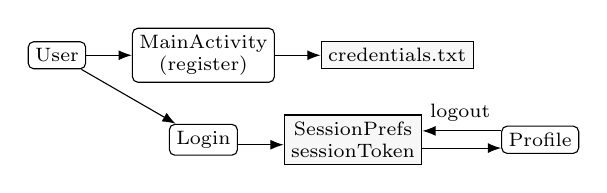
\begin{tikzpicture}[
  node distance=0.52cm and 0.58cm,
  box/.style={draw, rounded corners=2pt, align=center, font=\scriptsize, inner sep=2.5pt},
  data/.style={draw, align=center, font=\scriptsize, inner sep=2.5pt, fill=black!3},
  flow/.style={-Latex, line width=0.4pt}
]
\node[box] (user) {User};
\node[box, right=of user] (main) {MainActivity\\(register)};
\node[data, right=of main] (cred) {credentials.txt};
\node[box, below=of main] (login) {Login};
\node[data, right=of login] (prefs) {SessionPrefs\\sessionToken};
\node[box, right=1.0cm of prefs] (profile) {Profile};

\draw[flow] (user) -- (main);
\draw[flow] (main) -- (cred);
\draw[flow] (user) -- (login);
\draw[flow] ([yshift=-1.8pt]login.east) -- ([yshift=-1.8pt]prefs.west);
\draw[flow] ([yshift=-3.0pt]prefs.east) -- ([yshift=-3.0pt]profile.west);
\draw[flow] ([yshift=3.2pt]profile.west) -- ([yshift=3.2pt]prefs.east);
\node[font=\scriptsize, fill=white, inner sep=0.6pt] at ($(profile.west)!0.52!(prefs.east)+(0,0.34)$) {logout};
\end{tikzpicture}
\caption{Simple system model and key data flows.}
\label{fig:model}
\end{figure}

\section{Method and Tooling}
We used AI-assisted workflow planning and static analysis tooling to inspect the APK. Primary analysis used Android SDK \texttt{apkanalyzer} to recover manifest, package tree, and smali-like method code.

\begin{table}[t]
\centering
\footnotesize
\setlength{\tabcolsep}{3pt}
\renewcommand{\arraystretch}{1.1}
\begin{tabularx}{\columnwidth}{@{}>{\raggedright\arraybackslash}p{0.56\columnwidth}>{\raggedright\arraybackslash}X@{}}
\toprule
\textbf{Location} & \textbf{Role of Randomness} \\
\midrule
\path{MainActivity.randomNumberGenerator()} & UI/debug random; not auth-critical. \\
\path{Login.generateSessionToken()} & Security-sensitive session token generation. \\
\bottomrule
\end{tabularx}
\caption{Randomness locations and security relevance.}
\label{tab:random}
\end{table}

\begin{figure}[t]
\centering

\includegraphics[width=\columnwidth,trim=20 10 300 10,clip]{login_snippet.png}
\caption{Decompiled login excerpt showing session-token generation with \texttt{java.util.Random}.}
\label{fig:login}
\end{figure}

\section{Vulnerability: Predictable Session Token Generation}
\textbf{Root cause.} In \path{Login.generateSessionToken()}, the code creates \path{new Random()} and repeatedly calls \path{nextInt(62)} to build a 16-character token (evidence in \path{Login.smali}, lines 337--383).

\textbf{Session use path.} After successful credential check, login calls \path{createSession()} and stores the generated token into \path{SharedPreferences} key \path{sessionToken} (\path{Login.smali} lines 414--433; \path{Login$1.smali} lines 123--137).

\textbf{Risk.} Session tokens are authentication artifacts. Using \path{java.util.Random} for this role weakens unpredictability and enables session impersonation attempts under realistic local attacker assumptions.

\textbf{Concrete attack scenario.}
\begin{enumerate}
\item Attacker gains local capability to inspect or modify app state.
\item Attacker targets login/session creation window and predicts candidate token values generated by \path{Random}.
\item Attacker replays or writes a valid-looking token into trusted local session storage.
\item App trusts local session state and grants profile access, causing impersonation risk.
\end{enumerate}

\section{Mitigation}
Replace \path{java.util.Random} with \path{java.security.SecureRandom} for session token generation (for example 128--256 bits, Base64 URL-safe encoding). Also enforce token validation at protected entry points (for example in \path{Profile.onCreate}) and redirect to login when session state is absent or invalid.

This mitigation works because \path{SecureRandom} is designed for security-sensitive unpredictability, and explicit authorization checks prevent trusting arbitrary local state.

\section{Conclusion}
The intended weakness is present: a predictable PRNG is used for session token generation. The issue is directly tied to authentication state and has a clear local attack path. A targeted change to \path{SecureRandom} plus strict session validation addresses the core risk.

\section{References}
\small
\begin{enumerate}
\item Oracle Java SE API, \textit{java.util.Random}.\\
\url{https://docs.oracle.com/en/java/javase/21/docs/api/java.base/java/util/Random.html}.
\item Oracle Java SE API, \textit{java.security.SecureRandom}.\\
\url{https://docs.oracle.com/en/java/javase/21/docs/api/java.base/java/security/SecureRandom.html}.
\item Android Developers, \textit{SharedPreferences}.\\
\url{https://developer.android.com/training/data-storage/shared-preferences}.
\end{enumerate}

\end{document}
